\section*{АЦП параллельного преобразования}
\addcontentsline{toc}{section}{АЦП параллельного преобразования}
\subsection*{Синтез}
\addcontentsline{toc}{subsection}{Синтез}

По заданию работы требовалось синтезировать и построить схему АЦП параллельного
преобразования на 2 разряда. Аналого-цифровое преобразование является операцией,
устанавливающей отношение двух величин – входной аналоговой Vi и эталонной Vr.
Цифровой сигнал преобразователя есть кодовое представление этого отношения. Если
выходной код преобразователя является n-разрядным, то число дискретных выходных
уровней равно $2^n$. В данном случае $n = 2$, а значит число выходных уровней равно 4.

В методе параллельного преобразования входной сигнал сравнивается одновременно со
всеми пороговыми уровнями с помощью компараторов, смещённых по уровню опорного
сигнала на один младший значащий разряд относительно друг друга. Смещение
обеспечивается за счёт использования прецизионного резистивного делителя. При подаче
аналогового сигнала на вход АЦП компараторы (сравнивающие устройства), смещённые
выше уровня входного сигнала, имеют на выходе логический ноль, а смещённые ниже этого
уровня – логическую единицу.

Сигналы с выходов компараторов через D триггеры подаются на комбинационную схему
(приоритетный шифратор), на выходе которой получается цифровой код входного
напряжения. Для четырёх выходных уровней справедлива следующая таблица состояния
приоритетного шифратора:

\vspace*{5mm}

\begin{center}
    \begin{tabular}{
        |>\centering m{1cm}
        |>\centering m{3cm}
        |>\centering m{3cm}
        |>{\centering\arraybackslash} m{3cm} |
    }
        \hline
        $U_{\text{ВХ}}$ & Десятичный эквивалент & Двоичный эквивалент & Состояние компараторов \rowend
        0 & 0 & 00 & 000 \rowend
        1 & 1 & 01 & 001 \rowend
        2 & 2 & 10 & 011 \rowend
        3 & 3 & 11 & 111 \rowend
    \end{tabular}
\end{center}

Для синтеза всей схемы оставалось синтезировать приоритетный шифратор. Для этого
была построена более подробная таблица с переключательными функциями.

\begin{center}
    \begin{tabular}{
        |>\centering m{1cm}
        |>\centering m{2cm}
        |>\centering m{2cm}
        |>\centering m{2cm}
        |>\centering m{2cm}
        |>{\centering\arraybackslash} m{2cm} |
    }
        \hline
        № & $X_2$ & $X_1$ & $X_0$ & $Z_1$ & $Z_0$ \rowend 
        0 & 0 & 0 & 0 & 0 & 0 \rowend 
        1 & 0 & 0 & 1 & 0 & 1 \rowend 
        2 & 0 & 1 & 1 & 1 & 0 \rowend 
        3 & 1 & 1 & 1 & 1 & 1 \rowend 
    \end{tabular}
\end{center}

Чтобы синтезировать приоритетный шифратор требовалось построить по данной
таблице аналитические функции для переключательных функций $Z_10$ и $Z_1$, а затем полученные
функции минимизировать. Изначально были получены следующие переключательные
функции:

\begin{center}
    \begin{tabular}{
        l
    }
        $Z_0=X_0 \overline{X}_1 \overline{X}_2 + X_0X_1X_2$ \\[2mm]
        $Z_1=X_0X_1\overline{X}_2 + X_0X_1X_2=X_0X_1$
    \end{tabular}
\end{center}

\newpage

Таким образом, схема АЦП параллельного преобразования была построена:

\begin{figure*}[h!]
    \centering
    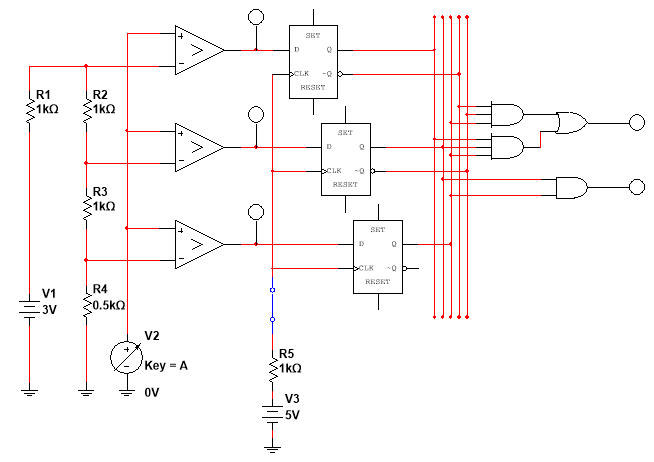
\includegraphics[scale=0.8]{images/image-1.png}
    \caption{АЦП параллельного преобразования}
\end{figure*}

\newpage

\subsection*{Тестирование}
\addcontentsline{toc}{subsection}{Тестирование}

Для проверки возьмем ненулевые наборы аналоговых значений. При смене диапозана будем подавать такт на триггеры
ожидая увидеть соответвующие значения выходных сигналов.

\begin{center}
    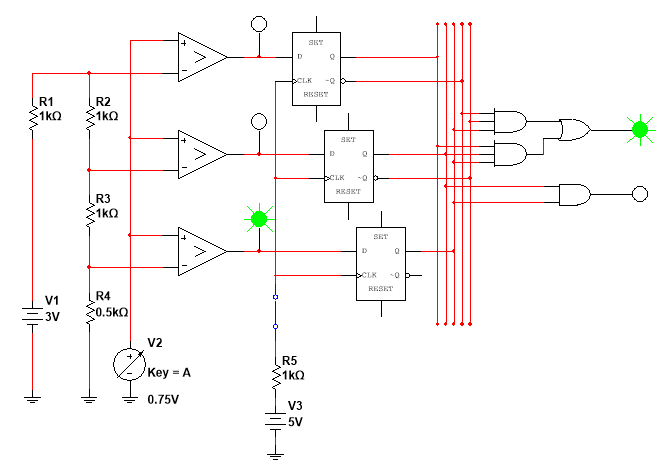
\includegraphics[width=.5\textwidth]{images/image-2.png}\hfill
    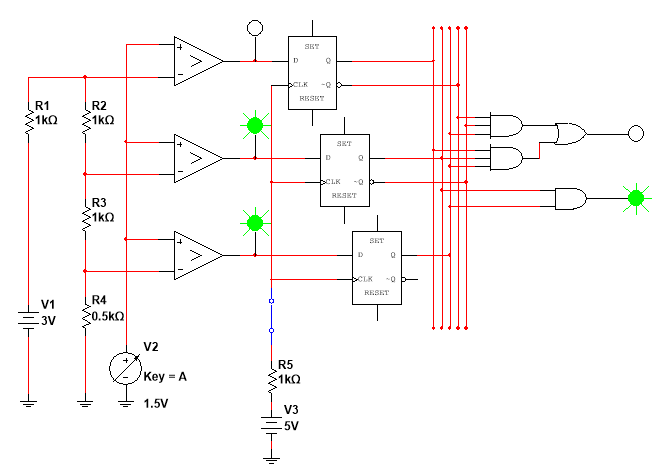
\includegraphics[width=.5\textwidth]{images/image-3.png}\hfill
    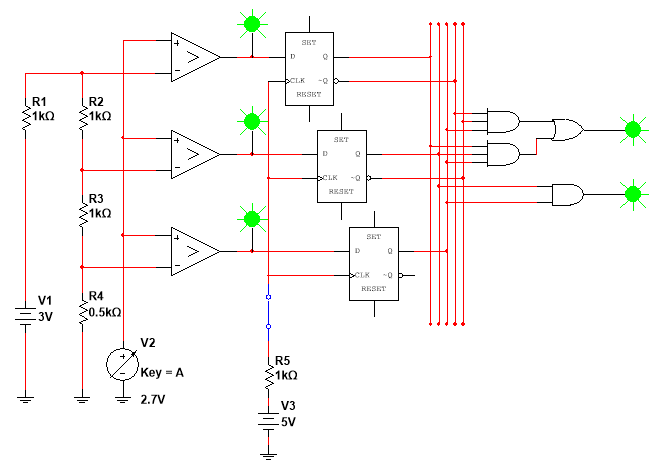
\includegraphics[width=.5\textwidth]{images/image-4.png}
\end{center}

Выходные сигналы соответствуют ожидаемым.